% Options for packages loaded elsewhere
\PassOptionsToPackage{unicode}{hyperref}
\PassOptionsToPackage{hyphens}{url}
\PassOptionsToPackage{dvipsnames,svgnames,x11names}{xcolor}
%
\documentclass[
  letterpaper,
  DIV=11,
  numbers=noendperiod]{scrartcl}

\usepackage{amsmath,amssymb}
\usepackage{iftex}
\ifPDFTeX
  \usepackage[T1]{fontenc}
  \usepackage[utf8]{inputenc}
  \usepackage{textcomp} % provide euro and other symbols
\else % if luatex or xetex
  \usepackage{unicode-math}
  \defaultfontfeatures{Scale=MatchLowercase}
  \defaultfontfeatures[\rmfamily]{Ligatures=TeX,Scale=1}
\fi
\usepackage{lmodern}
\ifPDFTeX\else  
    % xetex/luatex font selection
\fi
% Use upquote if available, for straight quotes in verbatim environments
\IfFileExists{upquote.sty}{\usepackage{upquote}}{}
\IfFileExists{microtype.sty}{% use microtype if available
  \usepackage[]{microtype}
  \UseMicrotypeSet[protrusion]{basicmath} % disable protrusion for tt fonts
}{}
\makeatletter
\@ifundefined{KOMAClassName}{% if non-KOMA class
  \IfFileExists{parskip.sty}{%
    \usepackage{parskip}
  }{% else
    \setlength{\parindent}{0pt}
    \setlength{\parskip}{6pt plus 2pt minus 1pt}}
}{% if KOMA class
  \KOMAoptions{parskip=half}}
\makeatother
\usepackage{xcolor}
\setlength{\emergencystretch}{3em} % prevent overfull lines
\setcounter{secnumdepth}{-\maxdimen} % remove section numbering
% Make \paragraph and \subparagraph free-standing
\makeatletter
\ifx\paragraph\undefined\else
  \let\oldparagraph\paragraph
  \renewcommand{\paragraph}{
    \@ifstar
      \xxxParagraphStar
      \xxxParagraphNoStar
  }
  \newcommand{\xxxParagraphStar}[1]{\oldparagraph*{#1}\mbox{}}
  \newcommand{\xxxParagraphNoStar}[1]{\oldparagraph{#1}\mbox{}}
\fi
\ifx\subparagraph\undefined\else
  \let\oldsubparagraph\subparagraph
  \renewcommand{\subparagraph}{
    \@ifstar
      \xxxSubParagraphStar
      \xxxSubParagraphNoStar
  }
  \newcommand{\xxxSubParagraphStar}[1]{\oldsubparagraph*{#1}\mbox{}}
  \newcommand{\xxxSubParagraphNoStar}[1]{\oldsubparagraph{#1}\mbox{}}
\fi
\makeatother

\usepackage{color}
\usepackage{fancyvrb}
\newcommand{\VerbBar}{|}
\newcommand{\VERB}{\Verb[commandchars=\\\{\}]}
\DefineVerbatimEnvironment{Highlighting}{Verbatim}{commandchars=\\\{\}}
% Add ',fontsize=\small' for more characters per line
\usepackage{framed}
\definecolor{shadecolor}{RGB}{241,243,245}
\newenvironment{Shaded}{\begin{snugshade}}{\end{snugshade}}
\newcommand{\AlertTok}[1]{\textcolor[rgb]{0.68,0.00,0.00}{#1}}
\newcommand{\AnnotationTok}[1]{\textcolor[rgb]{0.37,0.37,0.37}{#1}}
\newcommand{\AttributeTok}[1]{\textcolor[rgb]{0.40,0.45,0.13}{#1}}
\newcommand{\BaseNTok}[1]{\textcolor[rgb]{0.68,0.00,0.00}{#1}}
\newcommand{\BuiltInTok}[1]{\textcolor[rgb]{0.00,0.23,0.31}{#1}}
\newcommand{\CharTok}[1]{\textcolor[rgb]{0.13,0.47,0.30}{#1}}
\newcommand{\CommentTok}[1]{\textcolor[rgb]{0.37,0.37,0.37}{#1}}
\newcommand{\CommentVarTok}[1]{\textcolor[rgb]{0.37,0.37,0.37}{\textit{#1}}}
\newcommand{\ConstantTok}[1]{\textcolor[rgb]{0.56,0.35,0.01}{#1}}
\newcommand{\ControlFlowTok}[1]{\textcolor[rgb]{0.00,0.23,0.31}{\textbf{#1}}}
\newcommand{\DataTypeTok}[1]{\textcolor[rgb]{0.68,0.00,0.00}{#1}}
\newcommand{\DecValTok}[1]{\textcolor[rgb]{0.68,0.00,0.00}{#1}}
\newcommand{\DocumentationTok}[1]{\textcolor[rgb]{0.37,0.37,0.37}{\textit{#1}}}
\newcommand{\ErrorTok}[1]{\textcolor[rgb]{0.68,0.00,0.00}{#1}}
\newcommand{\ExtensionTok}[1]{\textcolor[rgb]{0.00,0.23,0.31}{#1}}
\newcommand{\FloatTok}[1]{\textcolor[rgb]{0.68,0.00,0.00}{#1}}
\newcommand{\FunctionTok}[1]{\textcolor[rgb]{0.28,0.35,0.67}{#1}}
\newcommand{\ImportTok}[1]{\textcolor[rgb]{0.00,0.46,0.62}{#1}}
\newcommand{\InformationTok}[1]{\textcolor[rgb]{0.37,0.37,0.37}{#1}}
\newcommand{\KeywordTok}[1]{\textcolor[rgb]{0.00,0.23,0.31}{\textbf{#1}}}
\newcommand{\NormalTok}[1]{\textcolor[rgb]{0.00,0.23,0.31}{#1}}
\newcommand{\OperatorTok}[1]{\textcolor[rgb]{0.37,0.37,0.37}{#1}}
\newcommand{\OtherTok}[1]{\textcolor[rgb]{0.00,0.23,0.31}{#1}}
\newcommand{\PreprocessorTok}[1]{\textcolor[rgb]{0.68,0.00,0.00}{#1}}
\newcommand{\RegionMarkerTok}[1]{\textcolor[rgb]{0.00,0.23,0.31}{#1}}
\newcommand{\SpecialCharTok}[1]{\textcolor[rgb]{0.37,0.37,0.37}{#1}}
\newcommand{\SpecialStringTok}[1]{\textcolor[rgb]{0.13,0.47,0.30}{#1}}
\newcommand{\StringTok}[1]{\textcolor[rgb]{0.13,0.47,0.30}{#1}}
\newcommand{\VariableTok}[1]{\textcolor[rgb]{0.07,0.07,0.07}{#1}}
\newcommand{\VerbatimStringTok}[1]{\textcolor[rgb]{0.13,0.47,0.30}{#1}}
\newcommand{\WarningTok}[1]{\textcolor[rgb]{0.37,0.37,0.37}{\textit{#1}}}

\providecommand{\tightlist}{%
  \setlength{\itemsep}{0pt}\setlength{\parskip}{0pt}}\usepackage{longtable,booktabs,array}
\usepackage{calc} % for calculating minipage widths
% Correct order of tables after \paragraph or \subparagraph
\usepackage{etoolbox}
\makeatletter
\patchcmd\longtable{\par}{\if@noskipsec\mbox{}\fi\par}{}{}
\makeatother
% Allow footnotes in longtable head/foot
\IfFileExists{footnotehyper.sty}{\usepackage{footnotehyper}}{\usepackage{footnote}}
\makesavenoteenv{longtable}
\usepackage{graphicx}
\makeatletter
\newsavebox\pandoc@box
\newcommand*\pandocbounded[1]{% scales image to fit in text height/width
  \sbox\pandoc@box{#1}%
  \Gscale@div\@tempa{\textheight}{\dimexpr\ht\pandoc@box+\dp\pandoc@box\relax}%
  \Gscale@div\@tempb{\linewidth}{\wd\pandoc@box}%
  \ifdim\@tempb\p@<\@tempa\p@\let\@tempa\@tempb\fi% select the smaller of both
  \ifdim\@tempa\p@<\p@\scalebox{\@tempa}{\usebox\pandoc@box}%
  \else\usebox{\pandoc@box}%
  \fi%
}
% Set default figure placement to htbp
\def\fps@figure{htbp}
\makeatother

\usepackage{booktabs}
\usepackage{caption}
\usepackage{longtable}
\usepackage{colortbl}
\usepackage{array}
\usepackage{anyfontsize}
\usepackage{multirow}
\KOMAoption{captions}{tableheading}
\makeatletter
\@ifpackageloaded{caption}{}{\usepackage{caption}}
\AtBeginDocument{%
\ifdefined\contentsname
  \renewcommand*\contentsname{Table of contents}
\else
  \newcommand\contentsname{Table of contents}
\fi
\ifdefined\listfigurename
  \renewcommand*\listfigurename{List of Figures}
\else
  \newcommand\listfigurename{List of Figures}
\fi
\ifdefined\listtablename
  \renewcommand*\listtablename{List of Tables}
\else
  \newcommand\listtablename{List of Tables}
\fi
\ifdefined\figurename
  \renewcommand*\figurename{Figure}
\else
  \newcommand\figurename{Figure}
\fi
\ifdefined\tablename
  \renewcommand*\tablename{Table}
\else
  \newcommand\tablename{Table}
\fi
}
\@ifpackageloaded{float}{}{\usepackage{float}}
\floatstyle{ruled}
\@ifundefined{c@chapter}{\newfloat{codelisting}{h}{lop}}{\newfloat{codelisting}{h}{lop}[chapter]}
\floatname{codelisting}{Listing}
\newcommand*\listoflistings{\listof{codelisting}{List of Listings}}
\makeatother
\makeatletter
\makeatother
\makeatletter
\@ifpackageloaded{caption}{}{\usepackage{caption}}
\@ifpackageloaded{subcaption}{}{\usepackage{subcaption}}
\makeatother

\usepackage{bookmark}

\IfFileExists{xurl.sty}{\usepackage{xurl}}{} % add URL line breaks if available
\urlstyle{same} % disable monospaced font for URLs
\hypersetup{
  pdftitle={Analysis},
  pdfauthor={Your Name},
  colorlinks=true,
  linkcolor={blue},
  filecolor={Maroon},
  citecolor={Blue},
  urlcolor={Blue},
  pdfcreator={LaTeX via pandoc}}


\title{Analysis}
\author{Your Name}
\date{2025-04-09}

\begin{document}
\maketitle

\renewcommand*\contentsname{Table of contents}
{
\hypersetup{linkcolor=}
\setcounter{tocdepth}{3}
\tableofcontents
}

\begin{Shaded}
\begin{Highlighting}[]
\FunctionTok{library}\NormalTok{(readxl)}
\FunctionTok{library}\NormalTok{(gt)}

\NormalTok{data }\OtherTok{=} \FunctionTok{read\_excel}\NormalTok{(}\StringTok{"data.xlsx"}\NormalTok{)}
\FunctionTok{colnames}\NormalTok{(data)}
\end{Highlighting}
\end{Shaded}

\begin{verbatim}
 [1] "sexo"                     "edad"                     "estado_civil"             "universidad"             
 [5] "grupo_carrera"            "ciclo"                    "promedio"                 "nse"                     
 [9] "roles"                    "vive_con"                 "ed_padre"                 "ed_madre"                
[13] "sit_laboral_padres"       "region"                   "tipo_universidad"         "fp_habilidadessociales1" 
[17] "fp_soportesocial2"        "fp_habilidadessociales3"  "fp_soportesocial4"        "fp_planear5"             
[21] "fp_metas6"                "fp_soportesocial7"        "fp_planear8"              "fp_metas9"               
[25] "fp_metas10"               "fp_metas11"               "fp_habilidadessociales12" "fp_habilidadessociales13"
[29] "fp_metas14"               "fp_planear15"             "fp_habilidadessociales16" "fp_habilidadessociales17"
[33] "fp_planear18"             "fp_metas19"               "fp_soportesocial20"       "fp_soportesocial21"      
[37] "fp_planear22"             "fp_soportesocial23"       "fp_planear24"             "fo_commitment2a"         
[41] "fo_commitment2b"          "fo_expectance2c"          "fo_exploration3.1"        "fo_exploration3.2"       
[45] "fo_commitment5a"          "fo_commitment5b"          "fo_commitment5c"          "fo_commitment6"          
[49] "fo_expectance7"           "fo_exploration8a"         "fo_exploration8b"         "fo_exploration8c"        
[53] "fo_exploration8d"         "fo_exploration8e"         "fo_internalcontrol9a"     "fo_internalcontrol9b"    
[57] "fo_internalcontrol9c"     "fo_internalcontrol9h"     "fo_expectance10a"         "fo_expectance10b"        
[61] "fo_expectance10c"         "fo_expectance10d"         "fo_expectance10e"         "fo_expectance10f"        
[65] "fo_value11a"              "fo_value11b"              "fo_value11c"              "fo_value11d"             
[69] "fo_value11e"              "fo_hopes3"                "fo_hopes4"                "fo_hopes8"               
[73] "fo_fears3"                "fo_fears4"                "fo_fears8"                "desercion"               
[77] "tutoria"                  "habilidades_sociales"     "soporte_social"           "planear"                 
[81] "metas"                    "internal_control"         "expectance"               "value"                   
[85] "hopes"                    "fears"                    "exploration"              "commitment"              
\end{verbatim}

\begin{Shaded}
\begin{Highlighting}[]
\NormalTok{corstars }\OtherTok{\textless{}{-}} \ControlFlowTok{function}\NormalTok{(x, }\AttributeTok{round\_digits =} \DecValTok{2}\NormalTok{, }\AttributeTok{use =} \StringTok{"pairwise.complete.obs"}\NormalTok{) \{}
  \FunctionTok{require}\NormalTok{(Hmisc)}
  
  \CommentTok{\# Compute correlation matrix with p{-}values}
\NormalTok{  rcorr\_res }\OtherTok{\textless{}{-}}\NormalTok{ Hmisc}\SpecialCharTok{::}\FunctionTok{rcorr}\NormalTok{(}\FunctionTok{as.matrix}\NormalTok{(x), }\AttributeTok{type =} \StringTok{"pearson"}\NormalTok{)}
\NormalTok{  r }\OtherTok{\textless{}{-}}\NormalTok{ rcorr\_res}\SpecialCharTok{$}\NormalTok{r}
\NormalTok{  p }\OtherTok{\textless{}{-}}\NormalTok{ rcorr\_res}\SpecialCharTok{$}\NormalTok{P}
  
  \CommentTok{\# Create significance stars}
\NormalTok{  stars }\OtherTok{\textless{}{-}} \FunctionTok{ifelse}\NormalTok{(p }\SpecialCharTok{\textless{}} \FloatTok{0.001}\NormalTok{, }\StringTok{"***"}\NormalTok{, }
           \FunctionTok{ifelse}\NormalTok{(p }\SpecialCharTok{\textless{}} \FloatTok{0.01}\NormalTok{, }\StringTok{"**"}\NormalTok{, }
           \FunctionTok{ifelse}\NormalTok{(p }\SpecialCharTok{\textless{}} \FloatTok{0.05}\NormalTok{, }\StringTok{"*"}\NormalTok{, }\StringTok{""}\NormalTok{)))}
  
  \CommentTok{\# Combine correlations and stars}
\NormalTok{  r\_stars }\OtherTok{\textless{}{-}} \FunctionTok{matrix}\NormalTok{(}\FunctionTok{paste0}\NormalTok{(}\FunctionTok{formatC}\NormalTok{(r, }\AttributeTok{format =} \StringTok{"f"}\NormalTok{, }\AttributeTok{digits =}\NormalTok{ round\_digits), stars), }
                    \AttributeTok{nrow =} \FunctionTok{nrow}\NormalTok{(r))}
  \FunctionTok{rownames}\NormalTok{(r\_stars) }\OtherTok{\textless{}{-}} \FunctionTok{colnames}\NormalTok{(x)}
  \FunctionTok{colnames}\NormalTok{(r\_stars) }\OtherTok{\textless{}{-}} \FunctionTok{colnames}\NormalTok{(x)}
  
  \CommentTok{\# Set diagonal to 1.00 without NA or stars}
  \FunctionTok{diag}\NormalTok{(r\_stars) }\OtherTok{\textless{}{-}} \FunctionTok{formatC}\NormalTok{(}\DecValTok{1}\NormalTok{, }\AttributeTok{format =} \StringTok{"f"}\NormalTok{, }\AttributeTok{digits =}\NormalTok{ round\_digits) }\CommentTok{\# Explicitly set diagonal to 1.00 without NA or stars}
  
  \CommentTok{\# Means and SDs}
\NormalTok{  means }\OtherTok{\textless{}{-}} \FunctionTok{sapply}\NormalTok{(x, }\ControlFlowTok{function}\NormalTok{(i) }\FunctionTok{mean}\NormalTok{(i, }\AttributeTok{na.rm =} \ConstantTok{TRUE}\NormalTok{))}
\NormalTok{  sds }\OtherTok{\textless{}{-}} \FunctionTok{sapply}\NormalTok{(x, }\ControlFlowTok{function}\NormalTok{(i) }\FunctionTok{sd}\NormalTok{(i, }\AttributeTok{na.rm =} \ConstantTok{TRUE}\NormalTok{))}
  
\NormalTok{  result }\OtherTok{\textless{}{-}} \FunctionTok{as.data.frame}\NormalTok{(r\_stars)}
\NormalTok{  result }\OtherTok{\textless{}{-}}\NormalTok{ tibble}\SpecialCharTok{::}\FunctionTok{rownames\_to\_column}\NormalTok{(result, }\AttributeTok{var =} \StringTok{"Variable"}\NormalTok{)}
\NormalTok{  result }\OtherTok{\textless{}{-}}\NormalTok{ dplyr}\SpecialCharTok{::}\FunctionTok{left\_join}\NormalTok{(}
\NormalTok{    tibble}\SpecialCharTok{::}\FunctionTok{tibble}\NormalTok{(}\AttributeTok{Variable =} \FunctionTok{names}\NormalTok{(means),}
                   \AttributeTok{Mean =} \FunctionTok{formatC}\NormalTok{(means, }\AttributeTok{digits =}\NormalTok{ round\_digits, }\AttributeTok{format =} \StringTok{"f"}\NormalTok{),}
                   \AttributeTok{SD =} \FunctionTok{formatC}\NormalTok{(sds, }\AttributeTok{digits =}\NormalTok{ round\_digits, }\AttributeTok{format =} \StringTok{"f"}\NormalTok{)),}
\NormalTok{    result,}
    \AttributeTok{by =} \StringTok{"Variable"}
\NormalTok{  )}
  
  \FunctionTok{return}\NormalTok{(result)}
\NormalTok{\}}
\end{Highlighting}
\end{Shaded}

\section{Limpieza de datos}\label{limpieza-de-datos}

\begin{Shaded}
\begin{Highlighting}[]
\NormalTok{data }\OtherTok{=}\NormalTok{ data }\SpecialCharTok{\%\textgreater{}\%} 
    \FunctionTok{mutate}\NormalTok{(}
        \AttributeTok{sexo =} \FunctionTok{ifelse}\NormalTok{(sexo }\SpecialCharTok{==} \StringTok{"Prefiero no decir"}\NormalTok{, }\ConstantTok{NA}\NormalTok{, sexo),}
        \AttributeTok{estado\_civil =} \FunctionTok{ifelse}\NormalTok{(estado\_civil }\SpecialCharTok{==} \StringTok{"NA"}\NormalTok{, }\ConstantTok{NA}\NormalTok{, estado\_civil),}
        \AttributeTok{estado\_civil =} \FunctionTok{ifelse}\NormalTok{(estado\_civil }\SpecialCharTok{==} \StringTok{\textquotesingle{}Soltero/a\textquotesingle{}}\NormalTok{, }\StringTok{"Soltero/a"}\NormalTok{, }\StringTok{"No Soltero"}\NormalTok{),}
        \AttributeTok{grupo\_carrera =} \FunctionTok{ifelse}\NormalTok{(grupo\_carrera }\SpecialCharTok{==} \StringTok{"NA"}\NormalTok{, }\ConstantTok{NA}\NormalTok{, grupo\_carrera),}
        \AttributeTok{promedio =} \FunctionTok{parse\_number}\NormalTok{(promedio),}
        \AttributeTok{nse =} \FunctionTok{ifelse}\NormalTok{(nse }\SpecialCharTok{==} \StringTok{\textquotesingle{}Bajo\textquotesingle{}}\NormalTok{, }\StringTok{"Bajo"}\NormalTok{, }\StringTok{"Medio/Alto"}\NormalTok{),}
        \AttributeTok{ed\_padre =} \FunctionTok{ifelse}\NormalTok{(ed\_padre }\SpecialCharTok{==} \StringTok{"NA"}\NormalTok{, }\ConstantTok{NA}\NormalTok{, ed\_padre),}
        \AttributeTok{ed\_madre =} \FunctionTok{ifelse}\NormalTok{(ed\_madre }\SpecialCharTok{==} \StringTok{"NA"}\NormalTok{, }\ConstantTok{NA}\NormalTok{, ed\_madre),}
        \AttributeTok{universidad =} \FunctionTok{ifelse}\NormalTok{(universidad }\SpecialCharTok{==} \StringTok{"NA"}\NormalTok{, }\ConstantTok{NA}\NormalTok{, universidad),}
        \AttributeTok{ed\_padre =} \FunctionTok{ifelse}\NormalTok{(ed\_padre }\SpecialCharTok{==} \StringTok{"sin educacion"}\NormalTok{, }\StringTok{"secundaria"}\NormalTok{, ed\_padre),}
        \AttributeTok{ed\_madre =} \FunctionTok{ifelse}\NormalTok{(ed\_madre }\SpecialCharTok{==} \StringTok{"sin educacion"}\NormalTok{, }\StringTok{"secundaria"}\NormalTok{, ed\_madre),}
        \AttributeTok{ed\_padre =} \FunctionTok{ifelse}\NormalTok{(ed\_padre }\SpecialCharTok{==} \StringTok{"secundaria"}\NormalTok{, }\StringTok{"secundaria o menos"}\NormalTok{, ed\_padre),}
        \AttributeTok{ed\_madre =} \FunctionTok{ifelse}\NormalTok{(ed\_madre }\SpecialCharTok{==} \StringTok{"secundaria"}\NormalTok{, }\StringTok{"secundaria o menos"}\NormalTok{, ed\_madre)}
\NormalTok{        ) }\SpecialCharTok{\%\textgreater{}\%}
    \FunctionTok{mutate\_at}\NormalTok{(}\FunctionTok{vars}\NormalTok{(desercion, habilidades\_sociales}\SpecialCharTok{:}\NormalTok{metas), parse\_number)}
\NormalTok{totales }\OtherTok{=}\NormalTok{ data }\SpecialCharTok{\%\textgreater{}\%} \FunctionTok{select}\NormalTok{(sexo}\SpecialCharTok{:}\NormalTok{tipo\_universidad, desercion, habilidades\_sociales}\SpecialCharTok{:}\NormalTok{metas)}
\end{Highlighting}
\end{Shaded}

He agrupado algunos datos, porque los tamaños de la muestra en cada
subgrupo son muy pequeños. Cuando no se usan para el analisis, los he
mantenido (e.g., \texttt{vive\_con},
\texttt{situacion\_laboral\_padres}).

\section{Datos para metodo}\label{datos-para-metodo}

\begin{Shaded}
\begin{Highlighting}[]
\NormalTok{totales }\SpecialCharTok{\%\textgreater{}\%} \FunctionTok{count}\NormalTok{(sexo)}
\end{Highlighting}
\end{Shaded}

\begin{verbatim}
# A tibble: 3 x 2
  sexo       n
  <chr>  <int>
1 Hombre   230
2 Mujer    532
3 <NA>       6
\end{verbatim}

\begin{Shaded}
\begin{Highlighting}[]
\FunctionTok{mean}\NormalTok{(totales}\SpecialCharTok{$}\NormalTok{edad)}
\end{Highlighting}
\end{Shaded}

\begin{verbatim}
[1] 21.45833
\end{verbatim}

\begin{Shaded}
\begin{Highlighting}[]
\FunctionTok{sd}\NormalTok{(totales}\SpecialCharTok{$}\NormalTok{edad)}
\end{Highlighting}
\end{Shaded}

\begin{verbatim}
[1] 2.538534
\end{verbatim}

\begin{Shaded}
\begin{Highlighting}[]
\FunctionTok{min}\NormalTok{(totales}\SpecialCharTok{$}\NormalTok{edad)}
\end{Highlighting}
\end{Shaded}

\begin{verbatim}
[1] 18
\end{verbatim}

\begin{Shaded}
\begin{Highlighting}[]
\FunctionTok{max}\NormalTok{(totales}\SpecialCharTok{$}\NormalTok{edad)}
\end{Highlighting}
\end{Shaded}

\begin{verbatim}
[1] 30
\end{verbatim}

\begin{Shaded}
\begin{Highlighting}[]
\NormalTok{totales }\SpecialCharTok{\%\textgreater{}\%} \FunctionTok{count}\NormalTok{(estado\_civil)}
\end{Highlighting}
\end{Shaded}

\begin{verbatim}
# A tibble: 3 x 2
  estado_civil     n
  <chr>        <int>
1 No Soltero      28
2 Soltero/a      736
3 <NA>             4
\end{verbatim}

\begin{Shaded}
\begin{Highlighting}[]
\NormalTok{totales }\SpecialCharTok{\%\textgreater{}\%} \FunctionTok{count}\NormalTok{(universidad)}
\end{Highlighting}
\end{Shaded}

\begin{verbatim}
# A tibble: 9 x 2
  universidad                                                n
  <chr>                                                  <int>
1 Pontificia Universidad Católica del Perú                 179
2 Universidad Católica de Santa María                      181
3 Universidad Católica de Trujillo Benedicto XVI           139
4 Universidad Nacional Agraria de la Selva - Tingo María    55
5 Universidad Nacional Jorge Basadre Grohmann               14
6 Universidad Nacional de San Martín                        18
7 Universidad Nacional de Ucayali                           59
8 Universidad Nacional de la Amazonía Peruana              122
9 <NA>                                                       1
\end{verbatim}

\begin{Shaded}
\begin{Highlighting}[]
\NormalTok{totales }\SpecialCharTok{\%\textgreater{}\%} \FunctionTok{count}\NormalTok{(grupo\_carrera)}
\end{Highlighting}
\end{Shaded}

\begin{verbatim}
# A tibble: 7 x 2
  grupo_carrera           n
  <chr>               <int>
1 arte y arquitectura    50
2 educación              27
3 gestion               155
4 humanidades            85
5 ingenieria            164
6 salud                 285
7 <NA>                    2
\end{verbatim}

\begin{Shaded}
\begin{Highlighting}[]
\NormalTok{totales }\SpecialCharTok{\%\textgreater{}\%} \FunctionTok{count}\NormalTok{(ciclo)}
\end{Highlighting}
\end{Shaded}

\begin{verbatim}
# A tibble: 9 x 2
  ciclo       n
  <chr>   <int>
1 Cuarto     64
2 Décimo     64
3 Noveno     78
4 Octavo     60
5 Quinto    119
6 Segundo    62
7 Sexto      75
8 Séptimo   111
9 Tercer    135
\end{verbatim}

\begin{Shaded}
\begin{Highlighting}[]
\FunctionTok{mean}\NormalTok{(totales}\SpecialCharTok{$}\NormalTok{promedio, }\AttributeTok{na.rm =}\NormalTok{ T)}
\end{Highlighting}
\end{Shaded}

\begin{verbatim}
[1] 14.74678
\end{verbatim}

\begin{Shaded}
\begin{Highlighting}[]
\FunctionTok{sd}\NormalTok{(totales}\SpecialCharTok{$}\NormalTok{promedio, }\AttributeTok{na.rm =}\NormalTok{ T)}
\end{Highlighting}
\end{Shaded}

\begin{verbatim}
[1] 1.810755
\end{verbatim}

\begin{Shaded}
\begin{Highlighting}[]
\FunctionTok{min}\NormalTok{(totales}\SpecialCharTok{$}\NormalTok{promedio, }\AttributeTok{na.rm =}\NormalTok{ T)}
\end{Highlighting}
\end{Shaded}

\begin{verbatim}
[1] 9.857
\end{verbatim}

\begin{Shaded}
\begin{Highlighting}[]
\FunctionTok{max}\NormalTok{(totales}\SpecialCharTok{$}\NormalTok{promedio, }\AttributeTok{na.rm =}\NormalTok{ T)}
\end{Highlighting}
\end{Shaded}

\begin{verbatim}
[1] 20
\end{verbatim}

\begin{Shaded}
\begin{Highlighting}[]
\NormalTok{totales }\SpecialCharTok{\%\textgreater{}\%} \FunctionTok{count}\NormalTok{(nse)}
\end{Highlighting}
\end{Shaded}

\begin{verbatim}
# A tibble: 2 x 2
  nse            n
  <chr>      <int>
1 Bajo         269
2 Medio/Alto   499
\end{verbatim}

\begin{Shaded}
\begin{Highlighting}[]
\NormalTok{totales }\SpecialCharTok{\%\textgreater{}\%} \FunctionTok{count}\NormalTok{(roles)}
\end{Highlighting}
\end{Shaded}

\begin{verbatim}
# A tibble: 2 x 2
  roles                 n
  <chr>             <int>
1 estudia y trabaja   447
2 solo estudia        321
\end{verbatim}

\begin{Shaded}
\begin{Highlighting}[]
\NormalTok{totales }\SpecialCharTok{\%\textgreater{}\%} \FunctionTok{count}\NormalTok{(vive\_con)}
\end{Highlighting}
\end{Shaded}

\begin{verbatim}
# A tibble: 4 x 2
  vive_con                                                         n
  <chr>                                                        <int>
1 Además de mi pareja y/o hijo(a)s, vivo con otros familiares     18
2 Además de mis padres y/o hermanos, vivo con otros familiares   150
3 Vivo con mi pareja y/o hijos                                    31
4 Vivo con mis padres y/o hermano(a)s                            569
\end{verbatim}

\begin{Shaded}
\begin{Highlighting}[]
\NormalTok{totales }\SpecialCharTok{\%\textgreater{}\%} \FunctionTok{count}\NormalTok{(ed\_padre)}
\end{Highlighting}
\end{Shaded}

\begin{verbatim}
# A tibble: 5 x 2
  ed_padre               n
  <chr>              <int>
1 post grado            67
2 secundaria o menos   234
3 tecnico              234
4 universitario        206
5 <NA>                  27
\end{verbatim}

\begin{Shaded}
\begin{Highlighting}[]
\NormalTok{totales }\SpecialCharTok{\%\textgreater{}\%} \FunctionTok{count}\NormalTok{(ed\_madre)}
\end{Highlighting}
\end{Shaded}

\begin{verbatim}
# A tibble: 5 x 2
  ed_madre               n
  <chr>              <int>
1 post grado            61
2 secundaria o menos   239
3 tecnico              279
4 universitario        181
5 <NA>                   8
\end{verbatim}

\begin{Shaded}
\begin{Highlighting}[]
\NormalTok{totales }\SpecialCharTok{\%\textgreater{}\%} \FunctionTok{count}\NormalTok{(sit\_laboral\_padres)}
\end{Highlighting}
\end{Shaded}

\begin{verbatim}
# A tibble: 4 x 2
  sit_laboral_padres        n
  <chr>                 <int>
1 No trabaja               35
2 Trabajo dependiente     353
3 Trabajo doméstico        43
4 Trabajo independiente   337
\end{verbatim}

\begin{Shaded}
\begin{Highlighting}[]
\NormalTok{totales }\SpecialCharTok{\%\textgreater{}\%} \FunctionTok{count}\NormalTok{(region)}
\end{Highlighting}
\end{Shaded}

\begin{verbatim}
# A tibble: 3 x 2
  region     n
  <chr>  <int>
1 costa    332
2 selva    254
3 sierra   182
\end{verbatim}

\begin{Shaded}
\begin{Highlighting}[]
\NormalTok{totales }\SpecialCharTok{\%\textgreater{}\%} \FunctionTok{count}\NormalTok{(tipo\_universidad)}
\end{Highlighting}
\end{Shaded}

\begin{verbatim}
# A tibble: 2 x 2
  tipo_universidad     n
  <chr>            <int>
1 privada            499
2 publica            269
\end{verbatim}

\section{Missing data}\label{missing-data}

Vamos a hacer listwise deletion. Voy a seleccionar todas las variables
que entran al analisis, y nos quedamos unicamente con los datos
completos.

Las variables demograficas que quedan son: \texttt{sexo} \texttt{edad}
\texttt{estado\_civil} \texttt{grupo\_carrera} \texttt{nse}
\texttt{ed\_padre} \texttt{ed\_madre} \texttt{region}
\texttt{tipo\_universidad}

\begin{Shaded}
\begin{Highlighting}[]
\NormalTok{totales }\OtherTok{=}\NormalTok{ totales }\SpecialCharTok{\%\textgreater{}\%} \FunctionTok{select}\NormalTok{(}\SpecialCharTok{{-}}\NormalTok{universidad, }\SpecialCharTok{{-}}\NormalTok{ciclo, }\SpecialCharTok{{-}}\NormalTok{roles, }\SpecialCharTok{{-}}\NormalTok{vive\_con, }\SpecialCharTok{{-}}\NormalTok{sit\_laboral\_padres) }\SpecialCharTok{\%\textgreater{}\%} \FunctionTok{drop\_na}\NormalTok{()}
\end{Highlighting}
\end{Shaded}

\section{Correlations}\label{correlations}

\begin{Shaded}
\begin{Highlighting}[]
\NormalTok{totales }\SpecialCharTok{\%\textgreater{}\%} \FunctionTok{select}\NormalTok{(edad, promedio, desercion}\SpecialCharTok{:}\NormalTok{metas) }\SpecialCharTok{\%\textgreater{}\%} \FunctionTok{corstars}\NormalTok{() }\SpecialCharTok{\%\textgreater{}\%} \FunctionTok{gt}\NormalTok{()}
\end{Highlighting}
\end{Shaded}

\begin{verbatim}
Loading required package: Hmisc
\end{verbatim}

\begin{verbatim}

Attaching package: 'Hmisc'
\end{verbatim}

\begin{verbatim}
The following object is masked from 'package:gt':

    html
\end{verbatim}

\begin{verbatim}
The following objects are masked from 'package:dplyr':

    src, summarize
\end{verbatim}

\begin{verbatim}
The following objects are masked from 'package:base':

    format.pval, units
\end{verbatim}

\begin{table}
\fontsize{12.0pt}{14.4pt}\selectfont
\begin{tabular*}{\linewidth}{@{\extracolsep{\fill}}lrrrrrrrrr}
\toprule
Variable & Mean & SD & edad & promedio & desercion & habilidades\_sociales & soporte\_social & planear & metas \\ 
\midrule\addlinespace[2.5pt]
edad & 21.33 & 2.52 & 1.00 & -0.15*** & 0.03 & 0.12** & -0.00 & 0.08 & 0.12** \\ 
promedio & 14.71 & 1.79 & -0.15*** & 1.00 & -0.11* & 0.02 & 0.16*** & 0.11* & 0.06 \\ 
desercion & 2.43 & 1.76 & 0.03 & -0.11* & 1.00 & -0.16*** & -0.17*** & -0.23*** & -0.23*** \\ 
habilidades\_sociales & 5.00 & 1.42 & 0.12** & 0.02 & -0.16*** & 1.00 & 0.50*** & 0.63*** & 0.71*** \\ 
soporte\_social & 4.81 & 1.19 & -0.00 & 0.16*** & -0.17*** & 0.50*** & 1.00 & 0.56*** & 0.55*** \\ 
planear & 5.19 & 1.25 & 0.08 & 0.11* & -0.23*** & 0.63*** & 0.56*** & 1.00 & 0.81*** \\ 
metas & 5.43 & 1.33 & 0.12** & 0.06 & -0.23*** & 0.71*** & 0.55*** & 0.81*** & 1.00 \\ 
\bottomrule
\end{tabular*}
\end{table}

\section{Proposed Model}\label{proposed-model}

\begin{Shaded}
\begin{Highlighting}[]
\FunctionTok{library}\NormalTok{(lavaan)}
\end{Highlighting}
\end{Shaded}

\begin{verbatim}
This is lavaan 0.6-19
lavaan is FREE software! Please report any bugs.
\end{verbatim}

\begin{Shaded}
\begin{Highlighting}[]
\NormalTok{model }\OtherTok{\textless{}{-}} \StringTok{\textquotesingle{}}
\StringTok{  \# Direct effects}
\StringTok{  metas \textasciitilde{} habilidades\_sociales + soporte\_social}
\StringTok{  planear \textasciitilde{} metas + habilidades\_sociales + soporte\_social + promedio}
\StringTok{  desercion \textasciitilde{} planear + promedio}
\StringTok{\textquotesingle{}}

\NormalTok{fit }\OtherTok{\textless{}{-}} \FunctionTok{sem}\NormalTok{(model, }\AttributeTok{data =}\NormalTok{ totales, }\AttributeTok{estimator =} \StringTok{"ML"}\NormalTok{, }\AttributeTok{missing =} \StringTok{"listwise"}\NormalTok{)}

\FunctionTok{summary}\NormalTok{(fit, }\AttributeTok{fit.measures =} \ConstantTok{TRUE}\NormalTok{, }\AttributeTok{standardized =} \ConstantTok{TRUE}\NormalTok{, }\AttributeTok{rsquare =} \ConstantTok{TRUE}\NormalTok{)}
\end{Highlighting}
\end{Shaded}

\begin{verbatim}
lavaan 0.6-19 ended normally after 1 iteration

  Estimator                                         ML
  Optimization method                           NLMINB
  Number of model parameters                        11

  Number of observations                           536

Model Test User Model:
                                                      
  Test statistic                                 5.356
  Degrees of freedom                                 4
  P-value (Chi-square)                           0.253

Model Test Baseline Model:

  Test statistic                              1087.486
  Degrees of freedom                                12
  P-value                                        0.000

User Model versus Baseline Model:

  Comparative Fit Index (CFI)                    0.999
  Tucker-Lewis Index (TLI)                       0.996

Loglikelihood and Information Criteria:

  Loglikelihood user model (H0)              -2314.362
  Loglikelihood unrestricted model (H1)      -2311.684
                                                      
  Akaike (AIC)                                4650.725
  Bayesian (BIC)                              4697.850
  Sample-size adjusted Bayesian (SABIC)       4662.933

Root Mean Square Error of Approximation:

  RMSEA                                          0.025
  90 Percent confidence interval - lower         0.000
  90 Percent confidence interval - upper         0.074
  P-value H_0: RMSEA <= 0.050                    0.748
  P-value H_0: RMSEA >= 0.080                    0.028

Standardized Root Mean Square Residual:

  SRMR                                           0.015

Parameter Estimates:

  Standard errors                             Standard
  Information                                 Expected
  Information saturated (h1) model          Structured

Regressions:
                   Estimate  Std.Err  z-value  P(>|z|)   Std.lv  Std.all
  metas ~                                                               
    habilidds_scls    0.538    0.031   17.100    0.000    0.538    0.574
    soporte_social    0.293    0.038    7.807    0.000    0.293    0.262
  planear ~                                                             
    metas             0.633    0.034   18.829    0.000    0.633    0.676
    habilidds_scls    0.072    0.030    2.371    0.018    0.072    0.082
    soporte_social    0.148    0.031    4.754    0.000    0.148    0.142
    promedio          0.033    0.017    1.917    0.055    0.033    0.047
  desercion ~                                                           
    planear          -0.307    0.059   -5.156    0.000   -0.307   -0.217
    promedio         -0.080    0.041   -1.941    0.052   -0.080   -0.082

Variances:
                   Estimate  Std.Err  z-value  P(>|z|)   Std.lv  Std.all
   .metas             0.801    0.049   16.371    0.000    0.801    0.452
   .planear           0.485    0.030   16.371    0.000    0.485    0.312
   .desercion         2.909    0.178   16.371    0.000    2.909    0.942

R-Square:
                   Estimate
    metas             0.548
    planear           0.688
    desercion         0.058
\end{verbatim}

\begin{Shaded}
\begin{Highlighting}[]
\FunctionTok{install.packages}\NormalTok{(}\StringTok{"semPlot"}\NormalTok{)}
\end{Highlighting}
\end{Shaded}

\begin{verbatim}

The downloaded binary packages are in
    /var/folders/vp/9bgcmjdd43s_01tpyt0dlk100000gr/T//Rtmps19vQh/downloaded_packages
\end{verbatim}

\begin{Shaded}
\begin{Highlighting}[]
\FunctionTok{library}\NormalTok{(semPlot)}

\FunctionTok{semPaths}\NormalTok{(fit, }\StringTok{"std"}\NormalTok{, }\AttributeTok{layout =} \StringTok{"tree"}\NormalTok{, }\AttributeTok{whatLabels =} \StringTok{"std"}\NormalTok{, }\AttributeTok{edge.label.cex =} \FloatTok{1.1}\NormalTok{)}
\end{Highlighting}
\end{Shaded}

\pandocbounded{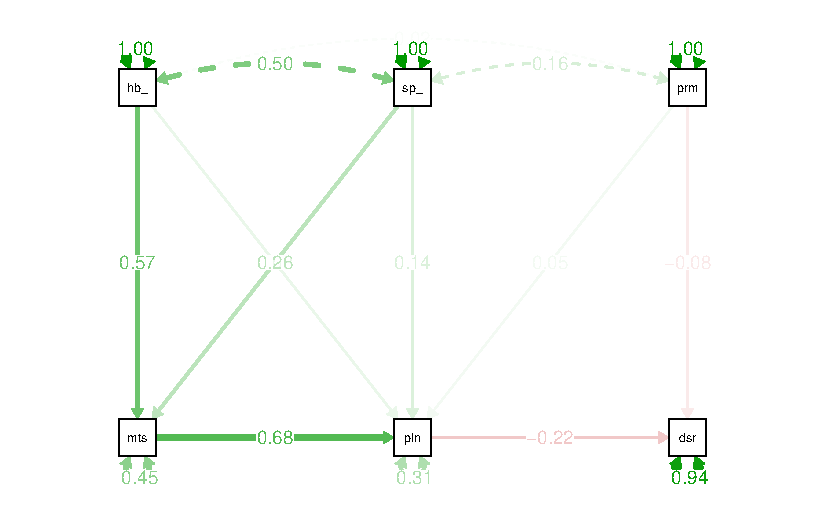
\includegraphics[keepaspectratio]{analysis_files/figure-pdf/unnamed-chunk-8-1.pdf}}

\begin{figure}[H]
\centering
\begin{tikzpicture}[>=stealth, node distance=2cm, on grid, auto]
  % Nodes
  \node[state] (ss) at (0,2) {Social\\Support};
  \node[state] (sk) at (0,5) {Social\\Skills};
  \node[state] (ge) at (3.5,3.5) {Goal-\\Efficacy};
  \node[state] (pl) at (7,3.5) {Planning};
  \node[state] (do) at (10.5,3.5) {Dropout\\Intention};
  \node[state] (gpa) at (7,1.3) {GPA};

  % Paths
  \path[->]
    (sk) edge node [sloped, above] {0.574} (ge)
    (ss) edge node [sloped, below] {0.262} (ge)
    (ge) edge node [above] {0.676} (pl)
    (sk) edge[bend left=15] node [above] {0.082} (pl)
    (ss) edge[bend right=15] node [below] {0.142} (pl)
    (gpa) edge node [right] {0.047} (pl)
    (pl) edge node [above] {-0.217} (do)
    (gpa) edge[bend left=20] node [below] {-0.082} (do);

\end{tikzpicture}
\caption{Standardized path model with goal-efficacy and planning predicting dropout intention.}
\end{figure}

\section{Demographic differences}\label{demographic-differences}

\begin{Shaded}
\begin{Highlighting}[]
\FunctionTok{library}\NormalTok{(dplyr)}
\FunctionTok{library}\NormalTok{(purrr)}
\FunctionTok{library}\NormalTok{(tidyr)}
\FunctionTok{library}\NormalTok{(broom)}
\FunctionTok{library}\NormalTok{(effectsize)}
\FunctionTok{library}\NormalTok{(stringr)}

\CommentTok{\# Grouping variables of interest}
\NormalTok{group\_vars }\OtherTok{\textless{}{-}} \FunctionTok{c}\NormalTok{(}
  \StringTok{"sexo"}\NormalTok{, }\StringTok{"estado\_civil"}\NormalTok{, }\StringTok{"grupo\_carrera"}\NormalTok{, }\StringTok{"region"}\NormalTok{, }\StringTok{"nse"}\NormalTok{,}
  \StringTok{"tipo\_universidad"}\NormalTok{, }\StringTok{"ed\_padre"}\NormalTok{, }\StringTok{"ed\_madre"}
\NormalTok{)}

\CommentTok{\# All numeric outcome variables}
\NormalTok{outcomes }\OtherTok{\textless{}{-}}\NormalTok{ totales }\SpecialCharTok{\%\textgreater{}\%} \FunctionTok{select}\NormalTok{(}\FunctionTok{where}\NormalTok{(is.numeric)) }\SpecialCharTok{\%\textgreater{}\%} \FunctionTok{select}\NormalTok{(}\SpecialCharTok{{-}}\NormalTok{edad) }\SpecialCharTok{\%\textgreater{}\%} \FunctionTok{names}\NormalTok{()}

\CommentTok{\# Function for pairwise comparisons}
\NormalTok{pairwise\_comparisons }\OtherTok{\textless{}{-}} \ControlFlowTok{function}\NormalTok{(group\_var, outcome) \{}
\NormalTok{  df }\OtherTok{\textless{}{-}}\NormalTok{ totales }\SpecialCharTok{\%\textgreater{}\%} \FunctionTok{select}\NormalTok{(}\FunctionTok{all\_of}\NormalTok{(}\FunctionTok{c}\NormalTok{(group\_var, outcome))) }\SpecialCharTok{\%\textgreater{}\%} \FunctionTok{drop\_na}\NormalTok{()}
\NormalTok{  df[[group\_var]] }\OtherTok{\textless{}{-}} \FunctionTok{as.factor}\NormalTok{(}\FunctionTok{str\_trim}\NormalTok{(df[[group\_var]]))  }\CommentTok{\# Ensure clean group names}
  
  \ControlFlowTok{if}\NormalTok{ (}\FunctionTok{length}\NormalTok{(}\FunctionTok{unique}\NormalTok{(df[[group\_var]])) }\SpecialCharTok{\textless{}} \DecValTok{2}\NormalTok{) }\FunctionTok{return}\NormalTok{(}\ConstantTok{NULL}\NormalTok{)}
  
  \CommentTok{\# Run ANOVA}
\NormalTok{  aov\_model }\OtherTok{\textless{}{-}} \FunctionTok{aov}\NormalTok{(}\FunctionTok{reformulate}\NormalTok{(group\_var, outcome), }\AttributeTok{data =}\NormalTok{ df)}
  
  \CommentTok{\# Tukey HSD}
\NormalTok{  tukey }\OtherTok{\textless{}{-}} \FunctionTok{TukeyHSD}\NormalTok{(aov\_model)[[}\DecValTok{1}\NormalTok{]] }\SpecialCharTok{\%\textgreater{}\%}
    \FunctionTok{as.data.frame}\NormalTok{() }\SpecialCharTok{\%\textgreater{}\%}
    \FunctionTok{rownames\_to\_column}\NormalTok{(}\StringTok{"Comparison"}\NormalTok{) }\SpecialCharTok{\%\textgreater{}\%}
    \FunctionTok{separate}\NormalTok{(Comparison, }\AttributeTok{into =} \FunctionTok{c}\NormalTok{(}\StringTok{"Group\_1"}\NormalTok{, }\StringTok{"Group\_2"}\NormalTok{), }\AttributeTok{sep =} \StringTok{"{-}"}\NormalTok{, }\AttributeTok{remove =} \ConstantTok{FALSE}\NormalTok{) }\SpecialCharTok{\%\textgreater{}\%}
    \FunctionTok{rename}\NormalTok{(}\AttributeTok{p =} \StringTok{\textasciigrave{}}\AttributeTok{p adj}\StringTok{\textasciigrave{}}\NormalTok{)  }\CommentTok{\# We\textquotesingle{}ll leave this unadjusted for now}
  
  \CommentTok{\# Get group stats}
\NormalTok{  group\_stats }\OtherTok{\textless{}{-}}\NormalTok{ df }\SpecialCharTok{\%\textgreater{}\%}
    \FunctionTok{group\_by}\NormalTok{(.data[[group\_var]]) }\SpecialCharTok{\%\textgreater{}\%}
    \FunctionTok{summarise}\NormalTok{(}
      \AttributeTok{mean =} \FunctionTok{mean}\NormalTok{(.data[[outcome]], }\AttributeTok{na.rm =} \ConstantTok{TRUE}\NormalTok{),}
      \AttributeTok{n =} \FunctionTok{n}\NormalTok{(),}
      \AttributeTok{.groups =} \StringTok{"drop"}
\NormalTok{    ) }\SpecialCharTok{\%\textgreater{}\%}
    \FunctionTok{rename}\NormalTok{(}\AttributeTok{Group =} \DecValTok{1}\NormalTok{, }\AttributeTok{Mean =}\NormalTok{ mean, }\AttributeTok{N =}\NormalTok{ n)}
  
  \CommentTok{\# Merge means}
\NormalTok{  tukey }\OtherTok{\textless{}{-}}\NormalTok{ tukey }\SpecialCharTok{\%\textgreater{}\%}
    \FunctionTok{left\_join}\NormalTok{(group\_stats, }\AttributeTok{by =} \FunctionTok{c}\NormalTok{(}\StringTok{"Group\_1"} \OtherTok{=} \StringTok{"Group"}\NormalTok{)) }\SpecialCharTok{\%\textgreater{}\%}
    \FunctionTok{rename}\NormalTok{(}\AttributeTok{Mean\_1 =}\NormalTok{ Mean, }\AttributeTok{N\_1 =}\NormalTok{ N) }\SpecialCharTok{\%\textgreater{}\%}
    \FunctionTok{left\_join}\NormalTok{(group\_stats, }\AttributeTok{by =} \FunctionTok{c}\NormalTok{(}\StringTok{"Group\_2"} \OtherTok{=} \StringTok{"Group"}\NormalTok{)) }\SpecialCharTok{\%\textgreater{}\%}
    \FunctionTok{rename}\NormalTok{(}\AttributeTok{Mean\_2 =}\NormalTok{ Mean, }\AttributeTok{N\_2 =}\NormalTok{ N)}
  
  \CommentTok{\# Compute d separately with safe handling}
\NormalTok{  d\_vals }\OtherTok{\textless{}{-}} \FunctionTok{map2\_dbl}\NormalTok{(tukey}\SpecialCharTok{$}\NormalTok{Group\_1, tukey}\SpecialCharTok{$}\NormalTok{Group\_2, }\ControlFlowTok{function}\NormalTok{(g1, g2) \{}
\NormalTok{    g1\_data }\OtherTok{\textless{}{-}}\NormalTok{ df }\SpecialCharTok{\%\textgreater{}\%} \FunctionTok{filter}\NormalTok{(.data[[group\_var]] }\SpecialCharTok{==}\NormalTok{ g1) }\SpecialCharTok{\%\textgreater{}\%} \FunctionTok{pull}\NormalTok{(outcome)}
\NormalTok{    g2\_data }\OtherTok{\textless{}{-}}\NormalTok{ df }\SpecialCharTok{\%\textgreater{}\%} \FunctionTok{filter}\NormalTok{(.data[[group\_var]] }\SpecialCharTok{==}\NormalTok{ g2) }\SpecialCharTok{\%\textgreater{}\%} \FunctionTok{pull}\NormalTok{(outcome)}
    \ControlFlowTok{if}\NormalTok{ (}\FunctionTok{length}\NormalTok{(g1\_data) }\SpecialCharTok{\textgreater{}} \DecValTok{1} \SpecialCharTok{\&\&} \FunctionTok{length}\NormalTok{(g2\_data) }\SpecialCharTok{\textgreater{}} \DecValTok{1}\NormalTok{) \{}
      \FunctionTok{tryCatch}\NormalTok{(}\FunctionTok{cohens\_d}\NormalTok{(g1\_data, g2\_data, }\AttributeTok{pooled =} \ConstantTok{TRUE}\NormalTok{)}\SpecialCharTok{$}\NormalTok{Cohens\_d, }\AttributeTok{error =} \ControlFlowTok{function}\NormalTok{(e) }\ConstantTok{NA}\NormalTok{)}
\NormalTok{    \} }\ControlFlowTok{else} \ConstantTok{NA}
\NormalTok{  \})}
  
  \CommentTok{\# Final table}
\NormalTok{  tukey }\SpecialCharTok{\%\textgreater{}\%}
    \FunctionTok{mutate}\NormalTok{(}
      \AttributeTok{Group\_Variable =}\NormalTok{ group\_var,}
      \AttributeTok{Outcome =}\NormalTok{ outcome,}
      \AttributeTok{d =} \FunctionTok{round}\NormalTok{(d\_vals, }\DecValTok{3}\NormalTok{),}
      \AttributeTok{Mean\_1 =} \FunctionTok{round}\NormalTok{(Mean\_1, }\DecValTok{3}\NormalTok{),}
      \AttributeTok{Mean\_2 =} \FunctionTok{round}\NormalTok{(Mean\_2, }\DecValTok{3}\NormalTok{),}
      \AttributeTok{N\_1 =}\NormalTok{ N\_1,}
      \AttributeTok{N\_2 =}\NormalTok{ N\_2,}
      \AttributeTok{p =} \FunctionTok{round}\NormalTok{(p, }\DecValTok{5}\NormalTok{)}
\NormalTok{    ) }\SpecialCharTok{\%\textgreater{}\%}
    \FunctionTok{select}\NormalTok{(Group\_Variable, Outcome, Group\_1, Group\_2,}
\NormalTok{           Mean\_1, Mean\_2, N\_1, N\_2, d, p)}
\NormalTok{\}}

\CommentTok{\# Run it across all variables}
\NormalTok{pairwise\_results }\OtherTok{\textless{}{-}} \FunctionTok{cross\_df}\NormalTok{(}\FunctionTok{list}\NormalTok{(}\AttributeTok{group\_var =}\NormalTok{ group\_vars, }\AttributeTok{outcome =}\NormalTok{ outcomes)) }\SpecialCharTok{\%\textgreater{}\%}
  \FunctionTok{pmap\_dfr}\NormalTok{(}\SpecialCharTok{\textasciitilde{}} \FunctionTok{pairwise\_comparisons}\NormalTok{(..}\DecValTok{1}\NormalTok{, ..}\DecValTok{2}\NormalTok{))}
\end{Highlighting}
\end{Shaded}

\begin{verbatim}
Warning: `cross_df()` was deprecated in purrr 1.0.0.
i Please use `tidyr::expand_grid()` instead.
i See <https://github.com/tidyverse/purrr/issues/768>.
\end{verbatim}

\begin{Shaded}
\begin{Highlighting}[]
\CommentTok{\# Apply p{-}value adjustment later}
\NormalTok{pairwise\_results }\OtherTok{\textless{}{-}}\NormalTok{ pairwise\_results }\SpecialCharTok{\%\textgreater{}\%}
  \FunctionTok{mutate}\NormalTok{(}\AttributeTok{p\_bh =} \FunctionTok{p.adjust}\NormalTok{(p, }\AttributeTok{method =} \StringTok{"bonferroni"}\NormalTok{)) }\SpecialCharTok{\%\textgreater{}\%}
  \FunctionTok{arrange}\NormalTok{(p\_bh)}

\CommentTok{\# View results}
\NormalTok{pairwise\_results }\SpecialCharTok{\%\textgreater{}\%} 
    \FunctionTok{as\_tibble}\NormalTok{() }\SpecialCharTok{\%\textgreater{}\%} 
    \FunctionTok{filter}\NormalTok{(p\_bh }\SpecialCharTok{\textless{}}\NormalTok{ .}\DecValTok{05}\NormalTok{) }\SpecialCharTok{\%\textgreater{}\%}
    \FunctionTok{ggplot}\NormalTok{(}\FunctionTok{aes}\NormalTok{(Group\_1, Group\_2, }\AttributeTok{fill =}\NormalTok{ d)) }\SpecialCharTok{+} 
\FunctionTok{geom\_tile}\NormalTok{() }\SpecialCharTok{+} 
\FunctionTok{facet\_wrap}\NormalTok{(}\SpecialCharTok{\textasciitilde{}}\NormalTok{Outcome)}
\end{Highlighting}
\end{Shaded}

\pandocbounded{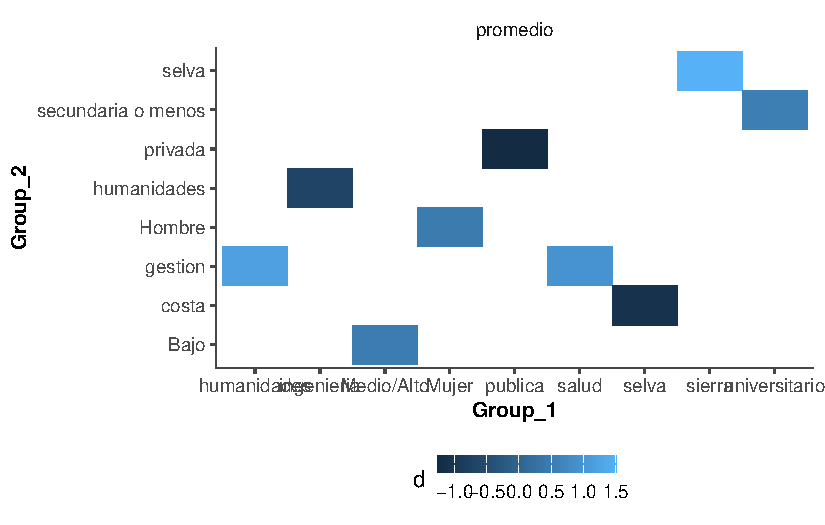
\includegraphics[keepaspectratio]{analysis_files/figure-pdf/unnamed-chunk-9-1.pdf}}

\begin{Shaded}
\begin{Highlighting}[]
\CommentTok{\# Table}
\NormalTok{pairwise\_results }\SpecialCharTok{\%\textgreater{}\%} 
    \FunctionTok{arrange}\NormalTok{(Group\_Variable) }\SpecialCharTok{\%\textgreater{}\%}
    \FunctionTok{group\_by}\NormalTok{(Outcome) }\SpecialCharTok{\%\textgreater{}\%}
    \FunctionTok{mutate}\NormalTok{(}\AttributeTok{Significant =} \FunctionTok{ifelse}\NormalTok{(p\_bh }\SpecialCharTok{\textless{}} \FloatTok{0.05}\NormalTok{, }\StringTok{"Yes"}\NormalTok{, }\StringTok{"No"}\NormalTok{)) }\SpecialCharTok{\%\textgreater{}\%}
    \FunctionTok{gt}\NormalTok{() }\SpecialCharTok{\%\textgreater{}\%}
    \FunctionTok{tab\_style}\NormalTok{(}
        \AttributeTok{style =} \FunctionTok{cell\_fill}\NormalTok{(}\AttributeTok{color =} \StringTok{"lightgreen"}\NormalTok{),}
        \AttributeTok{locations =} \FunctionTok{cells\_body}\NormalTok{(}
            \AttributeTok{columns =} \FunctionTok{c}\NormalTok{(p\_bh, Group\_1, Group\_2),}
            \AttributeTok{rows =}\NormalTok{ Significant }\SpecialCharTok{==} \StringTok{"Yes"}
\NormalTok{        )}
\NormalTok{    )}
\end{Highlighting}
\end{Shaded}

\begin{table}
\fontsize{12.0pt}{14.4pt}\selectfont
\begin{tabular*}{\linewidth}{@{\extracolsep{\fill}}lllrrrrrrrl}
\toprule
Group\_Variable & Group\_1 & Group\_2 & Mean\_1 & Mean\_2 & N\_1 & N\_2 & d & p & p\_bh & Significant \\ 
\midrule\addlinespace[2.5pt]
\multicolumn{11}{l}{promedio} \\[2.5pt] 
\midrule\addlinespace[2.5pt]
ed\_madre & {\cellcolor[HTML]{90EE90}{universitario}} & {\cellcolor[HTML]{90EE90}{secundaria o menos}} & 15.331 & 14.388 & 119 & 178 & 0.539 & 0.00005 & {\cellcolor[HTML]{90EE90}{0.01020}} & Yes \\ 
ed\_madre & universitario & tecnico & 15.331 & 14.627 & 119 & 201 & 0.391 & 0.00339 & 0.69156 & No \\ 
ed\_madre & secundaria o menos & post grado & 14.388 & 14.761 & 178 & 38 & -0.218 & 0.63666 & 1.00000 & No \\ 
ed\_madre & tecnico & post grado & 14.627 & 14.761 & 201 & 38 & -0.075 & 0.97357 & 1.00000 & No \\ 
ed\_madre & universitario & post grado & 15.331 & 14.761 & 119 & 38 & 0.308 & 0.30680 & 1.00000 & No \\ 
ed\_madre & tecnico & secundaria o menos & 14.627 & 14.388 & 201 & 178 & 0.139 & 0.55006 & 1.00000 & No \\ 
ed\_padre & secundaria o menos & post grado & 14.607 & 15.165 & 172 & 50 & -0.334 & 0.20970 & 1.00000 & No \\ 
ed\_padre & tecnico & post grado & 14.528 & 15.165 & 179 & 50 & -0.339 & 0.11652 & 1.00000 & No \\ 
ed\_padre & universitario & post grado & 14.927 & 15.165 & 135 & 50 & -0.132 & 0.85213 & 1.00000 & No \\ 
ed\_padre & tecnico & secundaria o menos & 14.528 & 14.607 & 179 & 172 & -0.044 & 0.97664 & 1.00000 & No \\ 
ed\_padre & universitario & secundaria o menos & 14.927 & 14.607 & 135 & 172 & 0.187 & 0.40137 & 1.00000 & No \\ 
ed\_padre & universitario & tecnico & 14.927 & 14.528 & 135 & 179 & 0.214 & 0.20457 & 1.00000 & No \\ 
estado\_civil & Soltero/a & No Soltero & 14.714 & 14.697 & 512 & 24 & 0.010 & 0.96348 & 1.00000 & No \\ 
grupo\_carrera & {\cellcolor[HTML]{90EE90}{humanidades}} & {\cellcolor[HTML]{90EE90}{gestion}} & 15.624 & 13.721 & 53 & 123 & 1.192 & 0.00000 & {\cellcolor[HTML]{90EE90}{0.00000}} & Yes \\ 
grupo\_carrera & {\cellcolor[HTML]{90EE90}{salud}} & {\cellcolor[HTML]{90EE90}{gestion}} & 15.256 & 13.721 & 197 & 123 & 0.941 & 0.00000 & {\cellcolor[HTML]{90EE90}{0.00000}} & Yes \\ 
grupo\_carrera & {\cellcolor[HTML]{90EE90}{ingenieria}} & {\cellcolor[HTML]{90EE90}{humanidades}} & 14.425 & 15.624 & 124 & 53 & -0.691 & 0.00022 & {\cellcolor[HTML]{90EE90}{0.04488}} & Yes \\ 
grupo\_carrera & salud & ingenieria & 15.256 & 14.425 & 197 & 124 & 0.487 & 0.00025 & 0.05100 & No \\ 
grupo\_carrera & educación & arte y arquitectura & 15.287 & 14.439 & 16 & 23 & 0.498 & 0.62671 & 1.00000 & No \\ 
grupo\_carrera & gestion & arte y arquitectura & 13.721 & 14.439 & 123 & 23 & -0.436 & 0.40869 & 1.00000 & No \\ 
grupo\_carrera & humanidades & arte y arquitectura & 15.624 & 14.439 & 53 & 23 & 0.772 & 0.05317 & 1.00000 & No \\ 
grupo\_carrera & ingenieria & arte y arquitectura & 14.425 & 14.439 & 124 & 23 & -0.008 & 1.00000 & 1.00000 & No \\ 
grupo\_carrera & salud & arte y arquitectura & 15.256 & 14.439 & 197 & 23 & 0.502 & 0.23173 & 1.00000 & No \\ 
grupo\_carrera & gestion & educación & 13.721 & 15.287 & 123 & 16 & -0.945 & 0.00610 & 1.00000 & No \\ 
grupo\_carrera & humanidades & educación & 15.624 & 15.287 & 53 & 16 & 0.218 & 0.98118 & 1.00000 & No \\ 
grupo\_carrera & ingenieria & educación & 14.425 & 15.287 & 124 & 16 & -0.472 & 0.37780 & 1.00000 & No \\ 
grupo\_carrera & salud & educación & 15.256 & 15.287 & 197 & 16 & -0.019 & 1.00000 & 1.00000 & No \\ 
grupo\_carrera & ingenieria & gestion & 14.425 & 13.721 & 124 & 123 & 0.404 & 0.01279 & 1.00000 & No \\ 
grupo\_carrera & salud & humanidades & 15.256 & 15.624 & 197 & 53 & -0.231 & 0.71312 & 1.00000 & No \\ 
nse & {\cellcolor[HTML]{90EE90}{Medio/Alto}} & {\cellcolor[HTML]{90EE90}{Bajo}} & 15.026 & 14.180 & 338 & 198 & 0.484 & 0.00000 & {\cellcolor[HTML]{90EE90}{0.00000}} & Yes \\ 
region & {\cellcolor[HTML]{90EE90}{selva}} & {\cellcolor[HTML]{90EE90}{costa}} & 13.556 & 15.206 & 208 & 191 & -1.115 & 0.00000 & {\cellcolor[HTML]{90EE90}{0.00000}} & Yes \\ 
region & {\cellcolor[HTML]{90EE90}{sierra}} & {\cellcolor[HTML]{90EE90}{selva}} & 15.784 & 13.556 & 137 & 208 & 1.515 & 0.00000 & {\cellcolor[HTML]{90EE90}{0.00000}} & Yes \\ 
region & sierra & costa & 15.784 & 15.206 & 137 & 191 & 0.354 & 0.00219 & 0.44676 & No \\ 
sexo & {\cellcolor[HTML]{90EE90}{Mujer}} & {\cellcolor[HTML]{90EE90}{Hombre}} & 14.978 & 14.168 & 361 & 175 & 0.461 & 0.00000 & {\cellcolor[HTML]{90EE90}{0.00000}} & Yes \\ 
tipo\_universidad & {\cellcolor[HTML]{90EE90}{publica}} & {\cellcolor[HTML]{90EE90}{privada}} & 13.560 & 15.492 & 216 & 320 & -1.269 & 0.00000 & {\cellcolor[HTML]{90EE90}{0.00000}} & Yes \\ 
\midrule\addlinespace[2.5pt]
\multicolumn{11}{l}{desercion} \\[2.5pt] 
\midrule\addlinespace[2.5pt]
ed\_madre & secundaria o menos & post grado & 2.449 & 2.658 & 178 & 38 & -0.113 & 0.91132 & 1.00000 & No \\ 
ed\_madre & tecnico & post grado & 2.373 & 2.658 & 201 & 38 & -0.159 & 0.79771 & 1.00000 & No \\ 
ed\_madre & universitario & post grado & 2.412 & 2.658 & 119 & 38 & -0.134 & 0.87687 & 1.00000 & No \\ 
ed\_madre & tecnico & secundaria o menos & 2.373 & 2.449 & 201 & 178 & -0.044 & 0.97494 & 1.00000 & No \\ 
ed\_madre & universitario & secundaria o menos & 2.412 & 2.449 & 119 & 178 & -0.022 & 0.99791 & 1.00000 & No \\ 
ed\_madre & universitario & tecnico & 2.412 & 2.373 & 119 & 201 & 0.023 & 0.99759 & 1.00000 & No \\ 
ed\_padre & secundaria o menos & post grado & 2.314 & 2.380 & 172 & 50 & -0.038 & 0.99552 & 1.00000 & No \\ 
ed\_padre & tecnico & post grado & 2.508 & 2.380 & 179 & 50 & 0.072 & 0.96853 & 1.00000 & No \\ 
ed\_padre & universitario & post grado & 2.481 & 2.380 & 135 & 50 & 0.055 & 0.98552 & 1.00000 & No \\ 
ed\_padre & tecnico & secundaria o menos & 2.508 & 2.314 & 179 & 172 & 0.113 & 0.72980 & 1.00000 & No \\ 
ed\_padre & universitario & secundaria o menos & 2.481 & 2.314 & 135 & 172 & 0.096 & 0.84167 & 1.00000 & No \\ 
ed\_padre & universitario & tecnico & 2.481 & 2.508 & 135 & 179 & -0.015 & 0.99914 & 1.00000 & No \\ 
estado\_civil & Soltero/a & No Soltero & 2.445 & 2.042 & 512 & 24 & 0.230 & 0.27226 & 1.00000 & No \\ 
grupo\_carrera & salud & humanidades & 2.020 & 3.151 & 197 & 53 & -0.675 & 0.00036 & 0.07344 & No \\ 
grupo\_carrera & salud & ingenieria & 2.020 & 2.766 & 197 & 124 & -0.441 & 0.00234 & 0.47736 & No \\ 
grupo\_carrera & educación & arte y arquitectura & 1.625 & 2.913 & 16 & 23 & -0.867 & 0.19473 & 1.00000 & No \\ 
grupo\_carrera & gestion & arte y arquitectura & 2.439 & 2.913 & 123 & 23 & -0.276 & 0.82984 & 1.00000 & No \\ 
grupo\_carrera & humanidades & arte y arquitectura & 3.151 & 2.913 & 53 & 23 & 0.121 & 0.99377 & 1.00000 & No \\ 
grupo\_carrera & ingenieria & arte y arquitectura & 2.766 & 2.913 & 124 & 23 & -0.079 & 0.99901 & 1.00000 & No \\ 
grupo\_carrera & salud & arte y arquitectura & 2.020 & 2.913 & 197 & 23 & -0.561 & 0.17325 & 1.00000 & No \\ 
grupo\_carrera & gestion & educación & 2.439 & 1.625 & 123 & 16 & 0.497 & 0.47791 & 1.00000 & No \\ 
grupo\_carrera & humanidades & educación & 3.151 & 1.625 & 53 & 16 & 0.830 & 0.02380 & 1.00000 & No \\ 
grupo\_carrera & ingenieria & educación & 2.766 & 1.625 & 124 & 16 & 0.638 & 0.12587 & 1.00000 & No \\ 
grupo\_carrera & salud & educación & 2.020 & 1.625 & 197 & 16 & 0.258 & 0.95004 & 1.00000 & No \\ 
grupo\_carrera & humanidades & gestion & 3.151 & 2.439 & 53 & 123 & 0.393 & 0.11966 & 1.00000 & No \\ 
grupo\_carrera & ingenieria & gestion & 2.766 & 2.439 & 124 & 123 & 0.183 & 0.66706 & 1.00000 & No \\ 
grupo\_carrera & salud & gestion & 2.020 & 2.439 & 197 & 123 & -0.258 & 0.27820 & 1.00000 & No \\ 
grupo\_carrera & ingenieria & humanidades & 2.766 & 3.151 & 124 & 53 & -0.200 & 0.74819 & 1.00000 & No \\ 
nse & Medio/Alto & Bajo & 2.373 & 2.520 & 338 & 198 & -0.084 & 0.34948 & 1.00000 & No \\ 
region & selva & costa & 2.462 & 2.450 & 208 & 191 & 0.006 & 0.99775 & 1.00000 & No \\ 
region & sierra & costa & 2.343 & 2.450 & 137 & 191 & -0.060 & 0.84982 & 1.00000 & No \\ 
region & sierra & selva & 2.343 & 2.462 & 137 & 208 & -0.068 & 0.81404 & 1.00000 & No \\ 
sexo & Mujer & Hombre & 2.269 & 2.754 & 361 & 175 & -0.278 & 0.00265 & 0.54060 & No \\ 
tipo\_universidad & publica & privada & 2.491 & 2.384 & 216 & 320 & 0.060 & 0.49277 & 1.00000 & No \\ 
\midrule\addlinespace[2.5pt]
\multicolumn{11}{l}{habilidades\_sociales} \\[2.5pt] 
\midrule\addlinespace[2.5pt]
ed\_madre & secundaria o menos & post grado & 5.086 & 4.649 & 178 & 38 & 0.303 & 0.31357 & 1.00000 & No \\ 
ed\_madre & tecnico & post grado & 5.040 & 4.649 & 201 & 38 & 0.264 & 0.40576 & 1.00000 & No \\ 
ed\_madre & universitario & post grado & 4.905 & 4.649 & 119 & 38 & 0.173 & 0.76904 & 1.00000 & No \\ 
ed\_madre & tecnico & secundaria o menos & 5.040 & 5.086 & 201 & 178 & -0.033 & 0.98898 & 1.00000 & No \\ 
ed\_madre & universitario & secundaria o menos & 4.905 & 5.086 & 119 & 178 & -0.132 & 0.70305 & 1.00000 & No \\ 
ed\_madre & universitario & tecnico & 4.905 & 5.040 & 119 & 201 & -0.096 & 0.84419 & 1.00000 & No \\ 
ed\_padre & secundaria o menos & post grado & 5.120 & 4.860 & 172 & 50 & 0.185 & 0.66410 & 1.00000 & No \\ 
ed\_padre & tecnico & post grado & 5.074 & 4.860 & 179 & 50 & 0.151 & 0.78049 & 1.00000 & No \\ 
ed\_padre & universitario & post grado & 4.790 & 4.860 & 135 & 50 & -0.049 & 0.99084 & 1.00000 & No \\ 
ed\_padre & tecnico & secundaria o menos & 5.074 & 5.120 & 179 & 172 & -0.032 & 0.99048 & 1.00000 & No \\ 
ed\_padre & universitario & secundaria o menos & 4.790 & 5.120 & 135 & 172 & -0.232 & 0.18076 & 1.00000 & No \\ 
ed\_padre & universitario & tecnico & 4.790 & 5.074 & 135 & 179 & -0.199 & 0.29480 & 1.00000 & No \\ 
estado\_civil & Soltero/a & No Soltero & 4.966 & 5.674 & 512 & 24 & -0.500 & 0.01699 & 1.00000 & No \\ 
grupo\_carrera & educación & arte y arquitectura & 4.990 & 5.145 & 16 & 23 & -0.121 & 0.99944 & 1.00000 & No \\ 
grupo\_carrera & gestion & arte y arquitectura & 5.091 & 5.145 & 123 & 23 & -0.042 & 0.99998 & 1.00000 & No \\ 
grupo\_carrera & humanidades & arte y arquitectura & 4.648 & 5.145 & 53 & 23 & -0.346 & 0.72759 & 1.00000 & No \\ 
grupo\_carrera & ingenieria & arte y arquitectura & 5.015 & 5.145 & 124 & 23 & -0.089 & 0.99863 & 1.00000 & No \\ 
grupo\_carrera & salud & arte y arquitectura & 5.006 & 5.145 & 197 & 23 & -0.103 & 0.99784 & 1.00000 & No \\ 
grupo\_carrera & gestion & educación & 5.091 & 4.990 & 123 & 16 & 0.074 & 0.99981 & 1.00000 & No \\ 
grupo\_carrera & humanidades & educación & 4.648 & 4.990 & 53 & 16 & -0.215 & 0.95948 & 1.00000 & No \\ 
grupo\_carrera & ingenieria & educación & 5.015 & 4.990 & 124 & 16 & 0.016 & 1.00000 & 1.00000 & No \\ 
grupo\_carrera & salud & educación & 5.006 & 4.990 & 197 & 16 & 0.012 & 1.00000 & 1.00000 & No \\ 
grupo\_carrera & humanidades & gestion & 4.648 & 5.091 & 53 & 123 & -0.313 & 0.40654 & 1.00000 & No \\ 
grupo\_carrera & ingenieria & gestion & 5.015 & 5.091 & 124 & 123 & -0.053 & 0.99834 & 1.00000 & No \\ 
grupo\_carrera & salud & gestion & 5.006 & 5.091 & 197 & 123 & -0.062 & 0.99543 & 1.00000 & No \\ 
grupo\_carrera & ingenieria & humanidades & 5.015 & 4.648 & 124 & 53 & 0.238 & 0.61777 & 1.00000 & No \\ 
grupo\_carrera & salud & humanidades & 5.006 & 4.648 & 197 & 53 & 0.250 & 0.58134 & 1.00000 & No \\ 
grupo\_carrera & salud & ingenieria & 5.006 & 5.015 & 197 & 124 & -0.006 & 1.00000 & 1.00000 & No \\ 
nse & Medio/Alto & Bajo & 4.983 & 5.022 & 338 & 198 & -0.027 & 0.76160 & 1.00000 & No \\ 
region & selva & costa & 5.159 & 5.044 & 208 & 191 & 0.083 & 0.69160 & 1.00000 & No \\ 
region & sierra & costa & 4.687 & 5.044 & 137 & 191 & -0.250 & 0.06334 & 1.00000 & No \\ 
region & sierra & selva & 4.687 & 5.159 & 137 & 208 & -0.334 & 0.00701 & 1.00000 & No \\ 
sexo & Mujer & Hombre & 4.971 & 5.051 & 361 & 175 & -0.056 & 0.54148 & 1.00000 & No \\ 
tipo\_universidad & publica & privada & 5.155 & 4.891 & 216 & 320 & 0.186 & 0.03488 & 1.00000 & No \\ 
\midrule\addlinespace[2.5pt]
\multicolumn{11}{l}{soporte\_social} \\[2.5pt] 
\midrule\addlinespace[2.5pt]
ed\_madre & secundaria o menos & post grado & 4.637 & 4.632 & 178 & 38 & 0.004 & 0.99999 & 1.00000 & No \\ 
ed\_madre & tecnico & post grado & 4.894 & 4.632 & 201 & 38 & 0.211 & 0.59591 & 1.00000 & No \\ 
ed\_madre & universitario & post grado & 4.968 & 4.632 & 119 & 38 & 0.290 & 0.42623 & 1.00000 & No \\ 
ed\_madre & tecnico & secundaria o menos & 4.894 & 4.637 & 201 & 178 & 0.215 & 0.15290 & 1.00000 & No \\ 
ed\_madre & universitario & secundaria o menos & 4.968 & 4.637 & 119 & 178 & 0.291 & 0.08720 & 1.00000 & No \\ 
ed\_madre & universitario & tecnico & 4.968 & 4.894 & 119 & 201 & 0.062 & 0.94962 & 1.00000 & No \\ 
ed\_padre & secundaria o menos & post grado & 4.681 & 4.827 & 172 & 50 & -0.116 & 0.87258 & 1.00000 & No \\ 
ed\_padre & tecnico & post grado & 4.833 & 4.827 & 179 & 50 & 0.006 & 0.99998 & 1.00000 & No \\ 
ed\_padre & universitario & post grado & 4.922 & 4.827 & 135 & 50 & 0.087 & 0.96260 & 1.00000 & No \\ 
ed\_padre & tecnico & secundaria o menos & 4.833 & 4.681 & 179 & 172 & 0.123 & 0.63015 & 1.00000 & No \\ 
ed\_padre & universitario & secundaria o menos & 4.922 & 4.681 & 135 & 172 & 0.202 & 0.29478 & 1.00000 & No \\ 
ed\_padre & universitario & tecnico & 4.922 & 4.833 & 135 & 179 & 0.077 & 0.91409 & 1.00000 & No \\ 
estado\_civil & Soltero/a & No Soltero & 4.800 & 4.944 & 512 & 24 & -0.121 & 0.56187 & 1.00000 & No \\ 
grupo\_carrera & educación & arte y arquitectura & 4.927 & 4.688 & 16 & 23 & 0.214 & 0.98992 & 1.00000 & No \\ 
grupo\_carrera & gestion & arte y arquitectura & 4.703 & 4.688 & 123 & 23 & 0.013 & 1.00000 & 1.00000 & No \\ 
grupo\_carrera & humanidades & arte y arquitectura & 4.541 & 4.688 & 53 & 23 & -0.138 & 0.99631 & 1.00000 & No \\ 
grupo\_carrera & ingenieria & arte y arquitectura & 4.868 & 4.688 & 124 & 23 & 0.150 & 0.98565 & 1.00000 & No \\ 
grupo\_carrera & salud & arte y arquitectura & 4.907 & 4.688 & 197 & 23 & 0.180 & 0.96145 & 1.00000 & No \\ 
grupo\_carrera & gestion & educación & 4.703 & 4.927 & 123 & 16 & -0.195 & 0.98111 & 1.00000 & No \\ 
grupo\_carrera & humanidades & educación & 4.541 & 4.927 & 53 & 16 & -0.338 & 0.86614 & 1.00000 & No \\ 
grupo\_carrera & ingenieria & educación & 4.868 & 4.927 & 124 & 16 & -0.047 & 0.99997 & 1.00000 & No \\ 
grupo\_carrera & salud & educación & 4.907 & 4.927 & 197 & 16 & -0.016 & 1.00000 & 1.00000 & No \\ 
grupo\_carrera & humanidades & gestion & 4.541 & 4.703 & 53 & 123 & -0.144 & 0.96203 & 1.00000 & No \\ 
grupo\_carrera & ingenieria & gestion & 4.868 & 4.703 & 124 & 123 & 0.139 & 0.88605 & 1.00000 & No \\ 
grupo\_carrera & salud & gestion & 4.907 & 4.703 & 197 & 123 & 0.170 & 0.67255 & 1.00000 & No \\ 
grupo\_carrera & ingenieria & humanidades & 4.868 & 4.541 & 124 & 53 & 0.273 & 0.54958 & 1.00000 & No \\ 
grupo\_carrera & salud & humanidades & 4.907 & 4.541 & 197 & 53 & 0.303 & 0.35219 & 1.00000 & No \\ 
grupo\_carrera & salud & ingenieria & 4.907 & 4.868 & 197 & 124 & 0.031 & 0.99976 & 1.00000 & No \\ 
nse & Medio/Alto & Bajo & 4.908 & 4.633 & 338 & 198 & 0.232 & 0.00989 & 1.00000 & No \\ 
region & selva & costa & 4.703 & 4.903 & 208 & 191 & -0.165 & 0.21439 & 1.00000 & No \\ 
region & sierra & costa & 4.828 & 4.903 & 137 & 191 & -0.063 & 0.84147 & 1.00000 & No \\ 
region & sierra & selva & 4.828 & 4.703 & 137 & 208 & 0.108 & 0.60304 & 1.00000 & No \\ 
sexo & Mujer & Hombre & 4.758 & 4.907 & 361 & 175 & -0.125 & 0.17500 & 1.00000 & No \\ 
tipo\_universidad & publica & privada & 4.728 & 4.859 & 216 & 320 & -0.111 & 0.20988 & 1.00000 & No \\ 
\midrule\addlinespace[2.5pt]
\multicolumn{11}{l}{planear} \\[2.5pt] 
\midrule\addlinespace[2.5pt]
ed\_madre & secundaria o menos & post grado & 5.256 & 4.816 & 178 & 38 & 0.377 & 0.19886 & 1.00000 & No \\ 
ed\_madre & tecnico & post grado & 5.206 & 4.816 & 201 & 38 & 0.293 & 0.28987 & 1.00000 & No \\ 
ed\_madre & universitario & post grado & 5.169 & 4.816 & 119 & 38 & 0.268 & 0.42444 & 1.00000 & No \\ 
ed\_madre & tecnico & secundaria o menos & 5.206 & 5.256 & 201 & 178 & -0.041 & 0.97990 & 1.00000 & No \\ 
ed\_madre & universitario & secundaria o menos & 5.169 & 5.256 & 119 & 178 & -0.073 & 0.93697 & 1.00000 & No \\ 
ed\_madre & universitario & tecnico & 5.169 & 5.206 & 119 & 201 & -0.028 & 0.99445 & 1.00000 & No \\ 
ed\_padre & secundaria o menos & post grado & 5.190 & 5.167 & 172 & 50 & 0.019 & 0.99944 & 1.00000 & No \\ 
ed\_padre & tecnico & post grado & 5.264 & 5.167 & 179 & 50 & 0.082 & 0.96250 & 1.00000 & No \\ 
ed\_padre & universitario & post grado & 5.088 & 5.167 & 135 & 50 & -0.060 & 0.98101 & 1.00000 & No \\ 
ed\_padre & tecnico & secundaria o menos & 5.264 & 5.190 & 179 & 172 & 0.061 & 0.94609 & 1.00000 & No \\ 
ed\_padre & universitario & secundaria o menos & 5.088 & 5.190 & 135 & 172 & -0.079 & 0.89235 & 1.00000 & No \\ 
ed\_padre & universitario & tecnico & 5.088 & 5.264 & 135 & 179 & -0.137 & 0.60491 & 1.00000 & No \\ 
estado\_civil & Soltero/a & No Soltero & 5.173 & 5.472 & 512 & 24 & -0.240 & 0.25144 & 1.00000 & No \\ 
grupo\_carrera & educación & arte y arquitectura & 5.135 & 4.928 & 16 & 23 & 0.149 & 0.99562 & 1.00000 & No \\ 
grupo\_carrera & gestion & arte y arquitectura & 5.245 & 4.928 & 123 & 23 & 0.275 & 0.87044 & 1.00000 & No \\ 
grupo\_carrera & humanidades & arte y arquitectura & 4.723 & 4.928 & 53 & 23 & -0.142 & 0.98624 & 1.00000 & No \\ 
grupo\_carrera & ingenieria & arte y arquitectura & 5.257 & 4.928 & 124 & 23 & 0.265 & 0.85213 & 1.00000 & No \\ 
grupo\_carrera & salud & arte y arquitectura & 5.265 & 4.928 & 197 & 23 & 0.288 & 0.82078 & 1.00000 & No \\ 
grupo\_carrera & gestion & educación & 5.245 & 5.135 & 123 & 16 & 0.090 & 0.99946 & 1.00000 & No \\ 
grupo\_carrera & humanidades & educación & 4.723 & 5.135 & 53 & 16 & -0.264 & 0.85400 & 1.00000 & No \\ 
grupo\_carrera & ingenieria & educación & 5.257 & 5.135 & 124 & 16 & 0.093 & 0.99912 & 1.00000 & No \\ 
grupo\_carrera & salud & educación & 5.265 & 5.135 & 197 & 16 & 0.107 & 0.99867 & 1.00000 & No \\ 
grupo\_carrera & humanidades & gestion & 4.723 & 5.245 & 53 & 123 & -0.409 & 0.10967 & 1.00000 & No \\ 
grupo\_carrera & ingenieria & gestion & 5.257 & 5.245 & 124 & 123 & 0.010 & 1.00000 & 1.00000 & No \\ 
grupo\_carrera & salud & gestion & 5.265 & 5.245 & 197 & 123 & 0.017 & 0.99999 & 1.00000 & No \\ 
grupo\_carrera & ingenieria & humanidades & 5.257 & 4.723 & 124 & 53 & 0.398 & 0.09483 & 1.00000 & No \\ 
grupo\_carrera & salud & humanidades & 5.265 & 4.723 & 197 & 53 & 0.432 & 0.05617 & 1.00000 & No \\ 
grupo\_carrera & salud & ingenieria & 5.265 & 5.257 & 197 & 124 & 0.007 & 1.00000 & 1.00000 & No \\ 
nse & Medio/Alto & Bajo & 5.207 & 5.152 & 338 & 198 & 0.045 & 0.61902 & 1.00000 & No \\ 
region & selva & costa & 5.304 & 5.071 & 208 & 191 & 0.191 & 0.14760 & 1.00000 & No \\ 
region & sierra & costa & 5.169 & 5.071 & 137 & 191 & 0.076 & 0.76025 & 1.00000 & No \\ 
region & sierra & selva & 5.169 & 5.304 & 137 & 208 & -0.111 & 0.58494 & 1.00000 & No \\ 
sexo & Mujer & Hombre & 5.159 & 5.243 & 361 & 175 & -0.067 & 0.46754 & 1.00000 & No \\ 
tipo\_universidad & publica & privada & 5.307 & 5.105 & 216 & 320 & 0.162 & 0.06605 & 1.00000 & No \\ 
\midrule\addlinespace[2.5pt]
\multicolumn{11}{l}{metas} \\[2.5pt] 
\midrule\addlinespace[2.5pt]
ed\_madre & secundaria o menos & post grado & 5.525 & 5.053 & 178 & 38 & 0.368 & 0.19449 & 1.00000 & No \\ 
ed\_madre & tecnico & post grado & 5.423 & 5.053 & 201 & 38 & 0.257 & 0.39571 & 1.00000 & No \\ 
ed\_madre & universitario & post grado & 5.401 & 5.053 & 119 & 38 & 0.242 & 0.49853 & 1.00000 & No \\ 
ed\_madre & tecnico & secundaria o menos & 5.423 & 5.525 & 201 & 178 & -0.080 & 0.87791 & 1.00000 & No \\ 
ed\_madre & universitario & secundaria o menos & 5.401 & 5.525 & 119 & 178 & -0.101 & 0.85858 & 1.00000 & No \\ 
ed\_madre & universitario & tecnico & 5.401 & 5.423 & 119 & 201 & -0.016 & 0.99891 & 1.00000 & No \\ 
ed\_padre & secundaria o menos & post grado & 5.424 & 5.463 & 172 & 50 & -0.029 & 0.99787 & 1.00000 & No \\ 
ed\_padre & tecnico & post grado & 5.524 & 5.463 & 179 & 50 & 0.047 & 0.99189 & 1.00000 & No \\ 
ed\_padre & universitario & post grado & 5.283 & 5.463 & 135 & 50 & -0.135 & 0.84590 & 1.00000 & No \\ 
ed\_padre & tecnico & secundaria o menos & 5.524 & 5.424 & 179 & 172 & 0.075 & 0.89673 & 1.00000 & No \\ 
ed\_padre & universitario & secundaria o menos & 5.283 & 5.424 & 135 & 172 & -0.104 & 0.79194 & 1.00000 & No \\ 
ed\_padre & universitario & tecnico & 5.283 & 5.524 & 135 & 179 & -0.180 & 0.38595 & 1.00000 & No \\ 
estado\_civil & Soltero/a & No Soltero & 5.410 & 5.757 & 512 & 24 & -0.260 & 0.21320 & 1.00000 & No \\ 
grupo\_carrera & educación & arte y arquitectura & 5.250 & 5.486 & 16 & 23 & -0.173 & 0.99438 & 1.00000 & No \\ 
grupo\_carrera & gestion & arte y arquitectura & 5.455 & 5.486 & 123 & 23 & -0.025 & 1.00000 & 1.00000 & No \\ 
grupo\_carrera & humanidades & arte y arquitectura & 5.110 & 5.486 & 53 & 23 & -0.265 & 0.87002 & 1.00000 & No \\ 
grupo\_carrera & ingenieria & arte y arquitectura & 5.534 & 5.486 & 124 & 23 & 0.037 & 0.99999 & 1.00000 & No \\ 
grupo\_carrera & salud & arte y arquitectura & 5.431 & 5.486 & 197 & 23 & -0.043 & 0.99997 & 1.00000 & No \\ 
grupo\_carrera & gestion & educación & 5.455 & 5.250 & 123 & 16 & 0.155 & 0.99238 & 1.00000 & No \\ 
grupo\_carrera & humanidades & educación & 5.110 & 5.250 & 53 & 16 & -0.085 & 0.99912 & 1.00000 & No \\ 
grupo\_carrera & ingenieria & educación & 5.534 & 5.250 & 124 & 16 & 0.198 & 0.96741 & 1.00000 & No \\ 
grupo\_carrera & salud & educación & 5.431 & 5.250 & 197 & 16 & 0.136 & 0.99525 & 1.00000 & No \\ 
grupo\_carrera & humanidades & gestion & 5.110 & 5.455 & 53 & 123 & -0.255 & 0.61550 & 1.00000 & No \\ 
grupo\_carrera & ingenieria & gestion & 5.534 & 5.455 & 124 & 123 & 0.060 & 0.99738 & 1.00000 & No \\ 
grupo\_carrera & salud & gestion & 5.431 & 5.455 & 197 & 123 & -0.019 & 0.99999 & 1.00000 & No \\ 
grupo\_carrera & ingenieria & humanidades & 5.534 & 5.110 & 124 & 53 & 0.295 & 0.38213 & 1.00000 & No \\ 
grupo\_carrera & salud & humanidades & 5.431 & 5.110 & 197 & 53 & 0.238 & 0.62732 & 1.00000 & No \\ 
grupo\_carrera & salud & ingenieria & 5.431 & 5.534 & 197 & 124 & -0.077 & 0.98535 & 1.00000 & No \\ 
nse & Medio/Alto & Bajo & 5.447 & 5.390 & 338 & 198 & 0.043 & 0.63314 & 1.00000 & No \\ 
region & selva & costa & 5.584 & 5.340 & 208 & 191 & 0.183 & 0.16077 & 1.00000 & No \\ 
region & sierra & costa & 5.304 & 5.340 & 137 & 191 & -0.026 & 0.96796 & 1.00000 & No \\ 
region & sierra & selva & 5.304 & 5.584 & 137 & 208 & -0.217 & 0.13564 & 1.00000 & No \\ 
sexo & Mujer & Hombre & 5.319 & 5.645 & 361 & 175 & -0.245 & 0.00795 & 1.00000 & No \\ 
tipo\_universidad & publica & privada & 5.595 & 5.311 & 216 & 320 & 0.214 & 0.01561 & 1.00000 & No \\ 
\bottomrule
\end{tabular*}
\end{table}




\end{document}
